\chapter{Technical Preliminaries}

This chapter has the goal of introducing the math and theory behind
formal languages, parsers, algebra, (zero knowledge) proofs of
knowledge, control and data flow in a program. Knowledge behind formal
languages is needed to design a parser which will later on be used to
create a custom compiler framework.

Zero knowledge proofs of knowledge are the basis of this thesis so
they need to be introduced here. First we start with group theory and
modular arithmetic, then we proceed with defining zero knowledge proofs
of knowledge and give a basic example of a protocol.

We conclude the chapter with introducing control flow graphs and data
flow (data dependency) graphs which are needed to reason about the
intermediate form the compiler generates.

\section{Formal Languages}

The theory of formal languages is needed to introduce a parser which
is the basic building block of a compiler. Here we give a short
overview of formal languages based on \cite{formal_languages} and for
a more detailed approach refer the reader to \cite{Hopcroft}.

We start with basic definitions of a formal language:

\begin{defn}[Alphabet]
  An alphabet $\Sigma$ is a set of symbols.
\end{defn}

\begin{defn}[String]
  A string over an alphabet $\Sigma$ is a sequence of symbols of $\Sigma$.
\end{defn}

\begin{defn}[Concatenation]
  Let $x = a_0 a_1 \dotsm a_n$ and $y = b_0 b_1 \dotsm b_n$, then the
  string $x y = a_0 a_1 \dotsm a_n b_0 b_1 \dotsm b_n$ is the
  concatenation of the strings $x$ and $y$.
\end{defn}

\begin{defn}[Sets]
  $\Sigma^*$ denotes the set of all the strings over the alphabet
  $\Sigma$. Likewise, $\Sigma^+$ denotes the set of all the non-empty
  strings over the alphabet $\Sigma$. $$\Sigma^+ \subseteq \Sigma^*
  \setminus \{ \epsilon \}$$ The empty set of strings is denoted
  $\emptyset$.
\end{defn}

\begin{defn}[Language]
  A language over the alphabet $\Sigma$ is a set of strings over
  $\Sigma$. Members of the language are called words of the language.
\end{defn}

\begin{defn}[Concatenation]
  Let $L_1$ and $L_2$ be two languages over alphabet $\Sigma$, the
  language $L_1 L_2 = \{x y | x \in L_1, y \in L_2 \}$ is the
  concatenation of $L_1$ and $L_2$.
\end{defn}

\begin{defn}[Kleene closure]
  Let $L$ be a language over $\Sigma$. Define 
  $$L^0 = \{ \epsilon \}$$
  $$L^i = L L^{i-1} \; \textrm{for} \; i \ge 1$$
  The \emph{Kleene closure} of $L$, denoted by $L^*$, is the language:
  $$ L^* = \bigcup_{i \ge 0} L^i $$
  the \emph{positive closure} is
  $$ L^+ = \bigcup_{i \ge 1} L^i $$
  It can be observed that
  $$ L^* = L^+ \cup \{ \epsilon \} $$
  $$ L^+ = L L^* $$
\end{defn}

We now have a formal basis to define a more powerful tool called
regular expressions. These regular expressions will allow us to
formally, yet compactly, specify the words of a language.

\subsection{Regular Expression}

When writing lexer rules for our compiler, we will need a language
that defines words of the language of our interest. Such a language is
called regular expressions and we briefly define it here:

\begin{defn}[Regular expression]
  A regular expression over $\Sigma$ is defined inductively as follows:
  \begin{enumerate}
  \item $\emptyset$ is a regular expression and represents the empty language
  \item $\epsilon$ is a regular expression and represents the language
    $L = \{ \epsilon \}$
  \item For each $c \in \Sigma$, $c$ is a regular expression and
    represents the language $L = \{ c \}$
  \item For any regular expressions $r$ of language $R$ and $s$ of language $S$:
    \begin{itemize}
    \item $r+s$ is a regular expression representing language $R \cup S$
    \item $r s$ is a regular expression representing language $R S$
    \item $r^*$ is a regular expression representing language $R^*$
    \item $r^+$ is a regular expression representing language $R^+$
    \end{itemize}
  \end{enumerate}
\end{defn}

\begin{thm}
  $r r^*$ can be represented as $r+$
\end{thm}

\begin{proof}
  $r r^*$ represents the language $R R^*$ which is $R^+$
\end{proof}

Now that we have the tool to specify the words of our language, we
need to specify the interactions between these words (e.g. which words
can follow a certain word, what the word ordering is). Such rules are
specified by grammars.

\subsection{Grammars}

When writing parser rules, we will need a language to specify the
interactions between the words of our language. Such a language
is called a grammar and we briefly define it here:

\begin{defn}[Grammar]
  A grammar is a 4-tuple $G = \left< \Sigma, V, S, P \right>$:
  \begin{enumerate}
  \item $\Sigma$ is a finite non-empty set called the \emph{terminal
    alphabet}. The elements of $\Sigma$ are called \emph{terminals}.
  \item $V$ is a finite non-empty set disjoint from $\Sigma$. The
    elements of $V$ are called \emph{non-terminals} or \emph{variables}.
  \item $S \in V$ is a distinguished symbol called the \emph{start symbol}
  \item $P$ is a finite set of \emph{productions (rules)} of the form
    $$ \alpha \rightarrow \beta $$
    $$ \alpha \in (\Sigma \cup V)^* V (\Sigma \cup V)^* $$
    $$ \beta \in (\Sigma \cup V)^* $$
  \end{enumerate}
\end{defn}

\begin{defn}[Context-free grammar]
  The grammar $G$ is a context free grammar iff $|\alpha|$ = 1 ($\alpha = V$).
\end{defn}

We now have all the tools to specify the input language of our
compiler. The parser of our compiler will transform an input file,
according to these rules, to a form suitable for further
processing. The forms we deal at this step are concrete syntax trees
and abstract syntax trees.

\subsection{Concrete Syntax Tree}

A Concrete Syntax Tree, also called a Parse Tree, is an ordered tree
representation of the input according to a given formal grammar.

For example, given the following input:
\begin{lstlisting}
a := b * c + d;
\end{lstlisting}
and the following grammar:
\begin{align*}
  \textrm{statement}  & \rightarrow \textrm{ID} := \textrm{expression} ; \\
  \textrm{expression} & \rightarrow \textrm{term} + \textrm{term} \\
  \textrm{term}       & \rightarrow \textrm{ID} * \textrm{ID} \\
  \textrm{term}       & \rightarrow \textrm{ID}
\end{align*}
the tree depicted in Figure \ref{fig:simple_cst} is a Concrete Syntax Tree.

\begin{figure}[hbt!]
  \centering
  \begin{tikzpicture}
    \Tree [.\node[language](statement){statement};
      [.\node[language](a){a};]
      [.\node[language](assign){:=};]
      [.\node[language](expression){expression};
        [.\node[language](term){term};
          [.\node[language](b){b};]
          [.\node[language](mul){*}; ]
          [.\node[language](c){c};]
        ]
        [.\node[language](plus){+};]
        [.\node[language](term2){term};
          [.\node[language](d){d};]
        ]
      ]
      [.\node[language](semi){;};]
    ]
  \end{tikzpicture}
  \caption{Concrete Syntax tree for a simple input and a simple grammar}
  \label{fig:simple_cst}
\end{figure}

\subsection{Abstract Syntax Tree}

An Abstract Syntax Tree (AST) is a tree representation of the abstract
syntax of the input. Given the same example
\begin{lstlisting}
a := b * c + d;
\end{lstlisting}
one possible variant of the tree is illustrated in Figure
\ref{fig:simple_ast}. Comparing it with the Parse Tree from Figure
\ref{fig:simple_cst} one can see that the choice of abstraction is
arbitrary.

\begin{figure}[hbt!]
  \centering
  \begin{tikzpicture}
    \Tree [.\node[language](equ){=};
      [.\node[language](a){a};]
      [.\node[language](add){+};
        [.\node[language](mul){*};
          [.\node[language](b){b};]
          [.\node[language](c){c};]
        ]
        [.\node[language](d){d};]
      ]
    ]
  \end{tikzpicture}
  \caption{An example AST for a simple expression}
  \label{fig:simple_ast}
\end{figure}

After all the definitions of the input and the output have been made,
it remains to define the actual tool transforming from the input to
the output. This tool is referred to as the parser.

\subsection{Parser}

Given a string $L$, satisfying grammar $G$, a parser tries to find the
derivation of $L$ from $S$. This derivation is the Concrete Syntax
Tree (Parse Tree). This derivation may further be abstracted into an
Abstract Syntax Tree that is easier for later manipulation. Figure
\ref{fig:parser_flow} shows the typical parser flow.

\begin{figure}[hbt!]
  \centering
  \begin{tikzpicture}[>=stealth,level distance=1.5cm,font=\tiny]
    \tikzstyle{edge from parent}=[draw,->]

    \Tree [.\node[language](input){Input};
      [.\node[compiler](parser){Parser};
        [.\node[language](ptree){Parse tree};
          [.\node[compiler](tgen){Tree generator};
            [.\node[language](ast){Abstract Syntax Tree};
            ]
          ]
        ]
      ]
    ]
  \end{tikzpicture}
  \caption{Parser flow}
  \label{fig:parser_flow}
\end{figure}

There are two approaches to parsing:
\begin{description}
\item[Top-down parsing] the derivation starts from the top (the root)
  of the parse tree and proceeds downwards.
\item[Bottom-up parsing] the derivation starts from the bottom (the
  leaves) of the parse tree and proceeds upwards.
\end{description}

The most popular top-down parser is an LL (left to right left-most
derivation) parser. The parser reads the input left to right and at
each step produces the left-most derivation of the input. Sub-types of
this parser include the symbol look-ahead which is the amount of next,
unseen symbols the parser can ``look at''. For example, an LL(1)
parser can only look 1 symbol ahead while an LL(*) parser is a parser
with arbitrary look-ahead.

\section{Group Theory and Modular Arithmetic}

Before we go into defining proofs of knowledge we need to define the
space we are operating on. We base our definitions on \cite{HAC}, but
the approach we take is a bit different. We choose to start with the
general and deduce the specific from it rather than taking an
inductive approach.

\begin{defn}[Group]
  A group $(G, \circ)$ is a set G with a binary operation $\circ$ defined on it
  that satisfies the following properties:
  \begin{enumerate}
  \item (Closure) $a, b \in G \implies a \circ b \in G$ 
  \item (Associativity) $(a \circ b) \circ c = a \circ (b \circ c)$ $\forall a,b,c \in G$
  \item (Identity element) $\exists I \in G$ such that $a \circ I = I \circ a = a$
  \item (Inverse element) ($\forall a \in G)(\exists a^{-1} \in G)$ such that $a \circ
    a^{-1} = a^{-1} \circ a = I$
  \end{enumerate}
\end{defn}

\begin{defn}[Abelian Group]
  A group $G$ is abelian iff $a \circ b = b \circ a$ $\forall a,b \in G$
\end{defn}

\begin{defn}[Finiteness and Order]
  A group $G$ is finite iff $|G|$ is finite. The number of elements in
  $G$ is called the \emph{order} of the group.
\end{defn}

\begin{defn}[Subgroup]
  A non-empty subset $H \subseteq G$ is a subgroup iff $H$ itself is a
  group w.r.t. to the binary operation of $G$. $H$ is a proper subgroup
  iff $H \neq G$.
\end{defn}

\begin{defn}[Cyclic Group]
  A group $G$ is cyclic iff $(\exists a \in G)(\forall b \in G)(i is
  Integer | b = a^i)$. Such an $a$ is called a generator of $G$. The
  group generated by $a$ is denoted as $\left< a \right>$.
\end{defn}

\begin{defn}[Order]
  Let $G$ be a group and $a \in G$. The order of $a$ is the least
  positive integer $t$ such that $a^t = I$, provided that such an
  integer exists.  If such an integer does not exist, the order is
  defined to be $\infty$.
\end{defn}

\begin{thm}[Lagrange's Theorem]
  If $G$ is a finite group and $H$ is a subgroup of $G$ then $|H|$ divides
  $|G|$.
\end{thm}

\begin{corr}
  The order of $a \in G$ divides $|G|$.
\end{corr}

\begin{defn}[Congruency]
  An integer $a$ is said to be congruent to integer $b$ modulo integer
  $n$, written $a \equiv b \pmod{n}$, iff $n$ divides $a-b$ (denoted as
  $n | a - b$). $n$ is called the \emph{modulus} of the congruency.
\end{defn}

\begin{defn}[Greatest Common Divisor]
  Given two integers $a$ and $b$, the greatest common divisor
  $d=\gcd(a,b)$ is the largest integer $d$ such that $d | a$ and $d | b$.
\end{defn}

\begin{defn}
  Two integers, $a$ and $b$, are relatively prime to each other iff
  \mbox{$\gcd(a,b)=1$}.
\end{defn}

\begin{defn}
  The integers modulo $n$, denoted $Z_n$, is the set of integers
  \mbox{$\{ 0,1,2,\ldots,n-1 \}$}.
\end{defn}

\begin{thm}
  Let $d = \gcd(a, n)$. Then the congruence equation $a x = b \pmod{n}$ has
  $d$ solutions $x$ iff $d$ divides $b$.
\end{thm}

\begin{corr}
  Let $a \in Z_n$. $a$ has a multiplicative inverse, denoted $a^{-1}$,
  iff \mbox{$\gcd(a, n) = 1$}.
\end{corr}

\begin{defn}
  The multiplicative group of $Z_n$ is $Z_n^* = \{a | \gcd(a,n) = 1
  \}$.  Specifically, if $n$ is prime, $Z_n^* = \{a | 1 \leq a \leq n-1
  \}$. The identity element of the multiplicative group is $1$.
\end{defn}

\begin{defn}
  The additive group of $Z_n$ is $Z_n^+ = \{a | 0 \leq a \leq n-1 \}$.
\end{defn}

\begin{defn}[Euler Phi Function]
  The Euler phi function, $\phi(n)$, also called Euler totient
  function, gives the number of integers from the interval $[1,n]$
  which are relatively prime to $n$.
\end{defn}

\begin{corr}
  The order of the group $Z_n^*$ is $\phi(n)$.
\end{corr}

\begin{corr}
  For a prime $p$, $\phi(p) = p-1$.
\end{corr}

\begin{corr}
  If $\gcd(m, n) = 1$, $\phi(m n) = \phi(m) \phi(n)$.
\end{corr}

\begin{thm}[Euler's Theorem]
  If $a \in Z_n^*$, then $a^{\phi(n)} = 1 \pmod{n}$.
\end{thm}

\begin{corr}[Fermat's Theorem]
  If $a \in Z_p^*$, where $p$ is prime, then $a^{p-1} = 1 \pmod{p}$.  
\end{corr}

\begin{corr}
  $a \in Z_n^*$ is a generator of the group $Z_n^*$ iff the order of
  $a$ is $\phi(n)$. $a$ is also called a primitive element of $Z_n^*$
  then.
\end{corr}

After defining the space we are operating on, it remains to define the
basis of this thesis, zero knowledge proofs of knowledge.

\section{Zero Knowledge Proofs of Knowledge}

Zero knowledge proofs of knowledge give us a powerful tool that allows
us to prove knowledge of a secret without actually revealing the
secret.  Here we need a more formal definition which we take from
\cite{Cameni98} and present as a brief overview. Some minor additions
were added for clarity.

\begin{defn}[Interactive Proof of Knowledge]
  Let $R \subseteq \{0,1\}^* \times \{0,1\}^*$ be a polinomially
  bounded binary relation and let $L_R$ be the language defined by
  $R$. An interactive proof of knowledge is a protocol $(P, V)$ that
  has the following properties:
  \begin{enumerate}
  \item (Completeness) $(x,w) \in R \implies [V, P(w)](x) = T$
  \item (Validity) There exists a probabilistic expected polynomial-time
    machine $K$ (Knowledge extractor) such that for every $\tilde{P}$, for
    all polynomials $f(\cdot)$ and all sufficiently large $x \in L_R$:
    \[
    p((x, K^{\tilde{P}(x)}) \in R) \geq p([V, \tilde{P}](x) = T) -
    \frac{1}{f(|x|)}
    \]
    The probabilities are taken over all random choices of $V$, $P$,
    $\tilde{P}$, $K$. The notation $\left[V, P(w)\right](x)$ denotes
    the protocol execution with the secret $x$ and the prover output
    $w$. $\tilde{P}$ includes malicious provers. $K^{\tilde{P}(x)}$
    denotes oracle access to $\tilde{P}(x)$. $f(\cdot)$ denotes the
    knowledge error.
  \end{enumerate}
\end{defn}

\begin{defn}[Soundness] $(\forall \tilde{P})(\forall x \notin
  L_R)(p([V, \tilde{P}](x) = T) < \frac{1}{2})$
\end{defn}
The additional soundness property is associated with $x \notin L_R$.  By
repeating the protocol many times, it can be made arbitrarily small
\cite{Cameni98}.

\begin{defn}[Indistinguishability]
  Let $L \in \{0,1\}^*$ be a language and let $A = \{A(x)\}_{x \in L}$
  and $B = \{B(x)\}_{x \in L}$ be two ensembles of random variables
  indexed by $L$. Ensembles $A$ and $B$ are:
  \begin{itemize}
  \item perfectly indistinguishable if for all $x \in L$ the variables
    $A(x)$ and $B(x)$ are identically distributed
  \item statistically indistinguishable if for every polynomial $f()$
    and for all sufficiently long $x \in L$:
    \[
    \sum_{\alpha \in \{0,1\}^*} | p(A(x) = \alpha) - p(B(x) = \alpha)|
    < \frac{1}{f(|x|)}
    \]
  \item computationally indistinguishable if for every probabilistic
    polynomial-time algorithm $D$, for every polynomial $f()$ and for
    all sufficiently long $x \in L$:
    \[
    |p(D(x, A(x) = 1) - p(D(x, B(x) = 1)| < \frac{1}{f(|x|)}
    \]
  \end{itemize}
\end{defn}

\begin{defn}[Zero-Knowledge]
  An interactive protocol $(P, V)$ is said to be
  perfectly/statistically/computationally zero-knowledge if for
  every probabilistic polynomial-time verifier $\tilde{V}$ there
  exists a probabilistic expected polynomial time simulator
  $S_{\tilde{V}}$ so that the two ensembles
  \[
  \{[\tilde{V}, P(w)](x)\}_{x \in L} \; \textrm{and} \; \{S_{\tilde{V}}(x)\}
  \]
  are perfectly/statistically/computationally indistinguishable.
\end{defn}

\begin{defn}[Honest Verifier Zero-Knowledge]
  An interactive protocol $(P, V)$ is said to be
  perfectly/statistically/computationally zero-knowledge if there
  exists a probabilistic expected polynomial time simulator
  $S_{\tilde{V}}$ so that the two ensembles
  \[
  \{[V, P(w)](x)\}_{x \in L} \; \textrm{and} \; \{S_V(x)\}
  \]
  are perfectly/statistically/computationally indistinguishable.
\end{defn}

To make a more practical definition we restrict to a subset of zero
knowledge proofs of knowledge called $\Sigma$-protocols.

\subsection{$\Sigma$-protocols}

A $\Sigma$-protocol is a three round honest verifier zero-knowledge
proof of knowledge \cite{cryptography_introduction}. The name comes
from the protocol's flow resemblance to the Greek letter $\Sigma$ as
shown in Figure \ref{fig:sigma_flow}. The rounds of the protocol are:
\begin{enumerate}
\item Commitment ($t$) - the prover commits to a value and sends that
  value to the verifier
\item Challenge ($c$) - the verifier computes a random challenge and asks
  the prover to output a value for that challenge
\item Response ($s$) - the prover responds with a new computed value
\end{enumerate}

\begin{figure}[h]
  \centering
  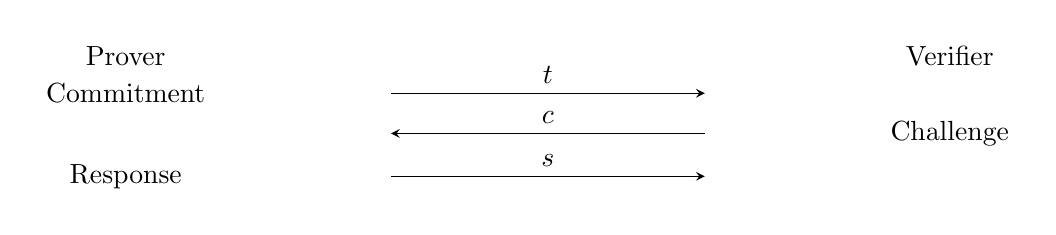
\begin{tikzpicture}[>=stealth]
    \node[matrix,column sep=2cm] {
      \node{\boxed{Prover}};                  &                           & &                             & \node{\boxed{Verifier}}; \\
      \node{Commitment};          & \node(commitment_s){}; & & \node(commitment_r){}; & \\
                                      & \node(challenge_r){}; & & \node(challenge_s){}; & \node{Challenge}; \\
      \node{Response}; & \node(response_s){}; & & \node(response_r){}; & \\
    };
    \draw[->] (commitment_s) -- (commitment_r) node[midway, anchor=south]{$t$};
    \draw[<-] (challenge_r) -- (challenge_s) node[midway, anchor=south]{$c$};
    \draw[->] (response_s) -- (response_r) node[midway, anchor=south]{$s$};
  \end{tikzpicture}
  \caption{Sigma protocol flow}
  \label{fig:sigma_flow}
\end{figure}

\subsubsection{Schnorr's Identification Protocol}
\label{subsubsec:schnorr_protocol}

A simple example of a $\Sigma$ protocol is Schnorr's Identification
Protocol \cite{schnorr_protocol, cryptography_introduction}. The
secret is a discrete logarithm $x$ of $y$ with respect to $g$ in some
finite group $G = \left< g \right>$ with prime order $q$, subgroup of
$Z_p^*$. The prover must prove knowledge of this secret to a verifier
under the homomorphism $f(a) : Z_q^+ \rightarrow G \subset Z_p^* :=
g^a$. Figure \ref{fig:schnorr_steps} gives an overview of the protocol
execution.

\begin{figure}[h]
  \centering
  \begin{tikzpicture}[>=stealth]
    \node[matrix,column sep=2cm] {
      \node{\boxed{Prover}};                  &                           & &                             & \node{\boxed{Verifier}}; \\
      \node{$r_1 \in Z_q^+$};                   &                           & &                             &                   \\
      \node{$t_1 = g^{r_1}$};          & \node(prover_round1_s){}; & & \node(verifier_round1_r){}; & \\
                                      & \node(prover_round2_r){}; & & \node(verifier_round1_s){}; & \node{$c \in \{0,1\}^*$}; \\
      \node{$s_1 = r_1 + x \cdot c$}; & \node(prover_round2_s){}; & & \node(verifier_round2_r){}; & \\
                                      &                           & &                             & \node{$s_1 \stackrel{?}{\in} Z_q^+$}; \\
                                      &                           & &                             & \node{$t_1 y^c \stackrel{?}{=} g^{s_1}$}; \\
    };
    \draw[->] (prover_round1_s) -- (verifier_round1_r) node[midway, anchor=south]{$t_1$};
    \draw[<-] (prover_round2_r) -- (verifier_round1_s) node[midway, anchor=south]{$c$};
    \draw[->] (prover_round2_s) -- (verifier_round2_r) node[midway, anchor=south]{$s_1$};
  \end{tikzpicture}
  \caption{Schnorr's Identification Protocol}
  \label{fig:schnorr_steps}
\end{figure}

\subsubsection{Camenisch-Stadler Notation}
\label{subsubsec:camenisch_stadler}

A simple and popular notation for specifying Sigma protocols is the
Camenisch-Stadler notation \cite{camenisch_stadler}. The Schnorr
Identification Protocol can be represented by the following:
\[
  \textrm{ZPK}\left[ (x): y = g^x \right]
\]
meaning prove knowledge of $x$, using a zero knowledge proof of
knowledge, such that $y=g^x$.

\filbreak

\section{Data Flow Graph and Control Flow Graph}

Our compiler will generate an intermediate form used for detailed
processing. This form is supposed to represent all the operations of
the protocol and can be represented as a directed graph detailing the
flow of the program.

The protocol is input via a text-file and is inherently
sequential. This means that the operations are laid out one after the
other. This inherently imposed ordering need not be the only one and
to make a better ordering w.r.t. to some goal we need constructs that
will allow us to extract all the constraints on the ordering. We keep
the nodes representing the operations while we classify each of the
edges as either a Data Edge or a Control Edge:
\begin{defn}[Data Edge]
  A data edge is an ordered relation between two operations such that
  the output/result of one operation is the input to the other.
\end{defn}
\begin{defn}[Control Edge]
  A control edge is an ordered relation between two operations such
  that the second operation has to be executed after the first finishes
  executing.
\end{defn}

The resulting graph can be separated into two independent graphs called
a Data Flow Graph and a Control Flow Graph.

\begin{defn}[Data Flow Graph]
  A data flow graph is a graph of the nodes representing the
  operations connected by data edges.
\end{defn}

\begin{defn}
  A control flow graph is a graph of the nodes representing the
  operations connected by control edges.
\end{defn}

A Data Flow Graph (DFG) completely and uniquely specifies the
algorithm, whereas the Control Flow Graph (CFG) gives the actual
implementation of the algorithm. After extracting the DFG, a different
CFG can be constructed satisfying the constraints of the
DFG~\cite{Schaumont}.

%%% Local Variables: 
%%% TeX-PDF-mode: t
%%% TeX-master: "thesis"
%%% End: 
